\chapter{Game Design}
\label{chap:game_design}

\section{Obiettivo}
\label{obiettivo}

L’obiettivo del lavoro di Tesi è stato quello di portare un pubblico che non conosce la tematica, ma è abituato a determinati contesti, che dimostra un interesse, anche non spiccato, verso questo bagaglio culturale, a mostrare curiosità nei confronti del tema del pre-Cinema.

Il pubblico a cui si fa riferimento è quello di ragazzi tra gli 11 ed i 18 anni, frequentanti perciò la scuola media inferiore e superiore. Con lo sviluppo, negli ultimi decenni, di differenti tipologie di media e di canali di informazione, tale fascia di età risulta estremamente abituata a contesti ludici o altre definizioni di intrattenimento sviluppate in forma digitale.
Ogni scelta di design è stata perciò effettuata tenendo conto del pubblico fruitore del prodotto finale, cercando perciò di limitare l’uso di metafore di gioco, o meccaniche che potessero risultare troppo complesse per un pubblico giovane.
Nonostante i ragazzi in tale fascia di età abbiano mostrato familiarità con il mezzo videoludico, abbiamo notato varie capacità di approccio per quanto riguarda l’input e l’interfacciamento con il prodotto sviluppato. Abbiamo quindi ritenuto opportuno tener conto anche delle differenti abilità di gioco ed abitudini ad utilizzare differenti dispositivi di input, e di conseguenza a prendere delle scelte di design che fossero state coerenti con quest’aspetto.

Risulta importante specificare che l’obiettivo primario del lavoro non è stato quello di insegnare o inculcare concetti ai ragazzi fruitori del gioco. Un approccio del genere avrebbe portato il prodotto ad essere caratterizzato da una forma didascalica e didattica, che avrebbe rischiato di sortire persino l’effetto opposto nei confronti degli utenti del gioco, l’essere noioso e poco divertente, poco appetibile ad un pubblico giovane.
Si è data perciò particolare importanza alla scelta di meccaniche di gioco divertenti, ambientazioni che avessero generato curiosità e stupore ed un gameplay stimolante. Elementi accompagnati dalla possibilità di fruire di schede informative e contenuti inerenti la tematica che si è deciso di affrontare.

\subsection{Piattaforma di riferimento e momenti museali}
\label{sec:piattaforma_di_riferimento}

Una scelta cruciale nella produzione di una qualsiasi forma di videogioco, è quella relativa alle piattaforme per cui sviluppare il prodotto finale. Risulta evidente come tale scelta influenzi pesantemente ogni elemento di design, dalla caratterizzazione più o meno dettagliata delle ambientazioni all’interfacciamento dell’utente.

Una prima analisi è stata quella relativa ai momenti museali a cui poter far riferimento. Per momenti museali intendiamo gli intervalli temporali in relazione all’entrata del pubblico in museo:
\begin{itemize}
	\item \textbf{Pre-visita.} Sono quei momenti in cui il pubblico si incuriosisce riguardo l’ambito museale e si interessa di una possibile visita. Volantini, passaparola, pubblicità, sono elementi che influenzano e caratterizzano il momento della pre-visita.
	\item \textbf{Visita.}  È l’intervallo temporale che il pubblico trascorre all’interno del museo, viene caratterizzato perciò dai contenuti veri e propri, oltre che da tutti gli altri elementi presenti all’interno del museo.
	\item \textbf{Post-visita.} Sono i momenti successivi alla visita del museo. Sono direttamente correlati alla soddisfazione provata dal pubblico, che può consigliare la visita ad altre persone, oltre che svolgere attività coerenti al contesto museale e provare interesse nei confronti di ciò che ha visitato.
\end{itemize}
Si è innanzitutto valutata la possibilità di sviluppare un prodotto fruibile all’interno del museo. L’applicazione avrebbe perciò avuto lo scopo di accompagnare la visita, tramite dei piccoli giochi, che avrebbero permesso di osservare alcuni degli elementi, presenti all’interno del museo, da prospettive diverse, generando nel pubblico una maggiore curiosità riguardo argomenti che sarebbero potuti risultare noiosi o poco interessanti. Un prodotto con un simile approccio è naturalmente sviluppabile per dispositivi mobili.

Secondo una nostra ipotesi, avvalorata anche da una personale ricerca di mercato, applicazioni del genere risultano molto interessanti per fasce di età inferiori rispetto a quella di riferimento per il progetto di Tesi.
I bambini, infatti, risultano particolarmente attratti da applicazioni semplici, immediate e veloci che possono rendere più piacevole la visita al museo, anche in compagnia di amici.
Ci si è quindi concentrati nei due restanti momenti museali, quelli precedenti e successivi alla visita.

Risulta importante specificare che la scelta della piattaforma di riferimento è stata effettuata anche in base alle meccaniche di gioco che si sono delineate durante le fasi di design del gameplay.
Abbiamo valutato la possibilità di sviluppare un casual game per dispositivi mobili, ma tale scelta avrebbe portato ad un prodotto superficiale, che sarebbe potuto risultare troppo semplicistico per il tema da voler affrontare.

\begin{figure}%[h]
	\centering
	% left bottom right top
	%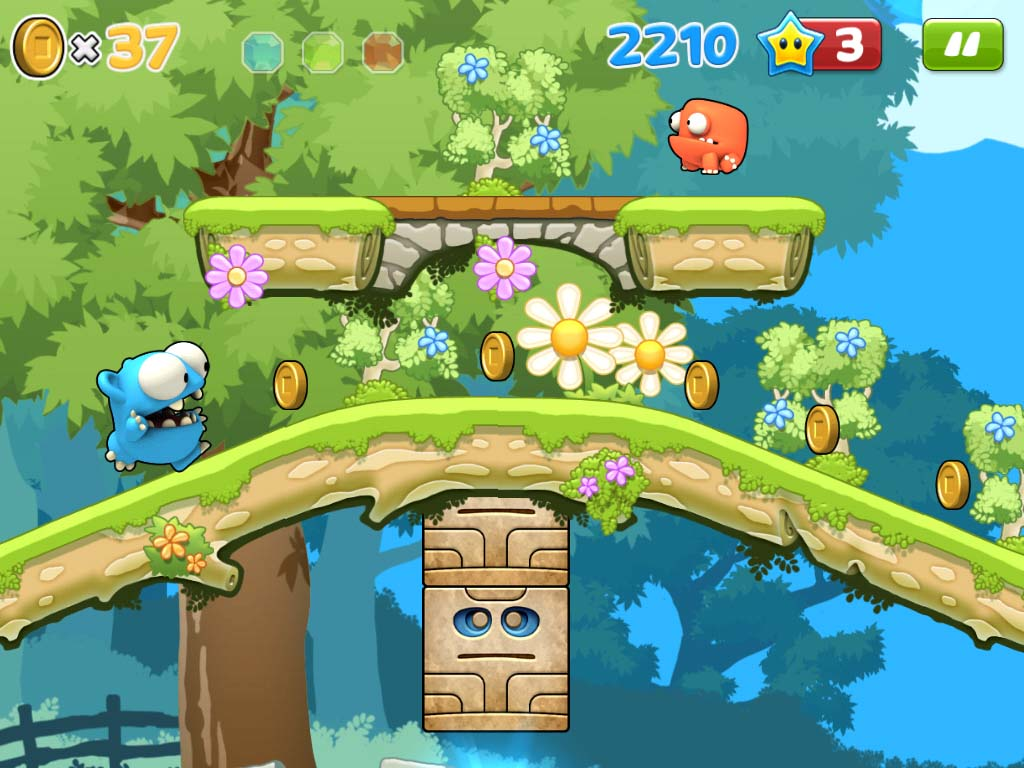
\includegraphics[clip= true, width= 0.8\columnwidth, trim= 1.5cm 3.0cm 0.6cm 0.0cm]{images/gameDesign/01_megarun.jpg}
	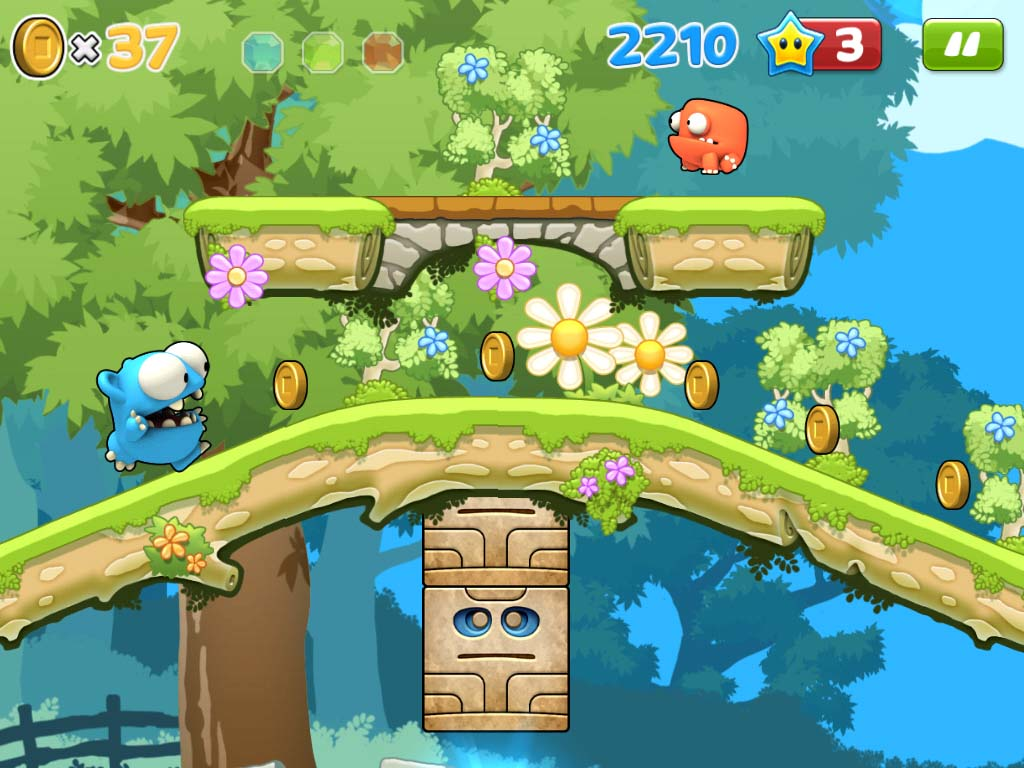
\includegraphics[width= 0.8\columnwidth]{images/gameDesign/01_megarun.jpg}
	\caption{Megarun: esempio di casual game.}
	\label{fig:casual_game}
\end{figure}

La natura platform/puzzle ideata durante le fasi di Design, ci ha spinto a sviluppare il prodotto per PC e console. Tali piattaforme permettono l’utilizzo di dispositivi di input più adatti alle tipologie di gameplay che sono state progettate, oltre che fornire una qualità visiva più consona all’estetica con cui si vuole caratterizzare il prodotto finito.
Tale scelta fornisce una ampia libertà di design, permettendo di sviluppare meccaniche complesse e profonde storyline, tipiche di una produzione di buon livello.

Concludendo, si è quindi scelto di sviluppare il videogioco per PC e console, con lo scopo di generare curiosità riguardo l’ambito del pre-cinema, attraverso meccaniche di gioco mirate, ambientazioni caratteristiche e schede informative studiate per fornire un buon supporto. Questo approccio risulta quindi coerente con i momenti museali di pre e post-visita, generando interesse nei confronti di un tema non ancora approfondito, o fornendo un buon metodo per osservare tematiche già note, apprese da una precedente visita, da un differente punto di vista.

\section{Meccaniche}
\label{sec:meccaniche}

Le meccaniche di gioco sono forse il nucleo più importante di una produzione videoludica di qualità, sono gli elementi che rimangono quando estetica, tecnologia e storia vengono meno, ed anche in queste condizioni, il prodotto, se caratterizzato da buone meccaniche, deve risultare piacevole ed efficace.
Il gameplay deve essere caratterizzato da regole semplici, ma allo stesso tempo flessibili, devono essere facili da capire, ma difficili da padroneggiare.

Il concetto di meccanica di gioco è strettamente legato a quello delle regole del game design, argomento che quindi non si limita ai videogiochi, ma a tutte le forme di intrattenimento che fanno riferimento al termine astratto di \textit{gioco}.
Abbiamo quindi fatto particolare attenzione al fornire al giocatore uno spazio di gioco in cui le meccaniche fornite avessero assicurato una sensazione di libertà, regolata però da limiti per circoscriverne le possibilità.
Il prodotto deve essere caratterizzato da pochi elementi di gameplay, ma che permettano al giocatore, entro certi limiti, di sentirsi libero di agire.

Ogni meccanica deve quindi essere semplice da capire e da utilizzare, ma deve richiedere un impegno ed uno studio progressivo per essere padroneggiata al meglio ed essere sfruttata in tutte le sue potenzialità.

Questo concetto è bene espresso nel libro \textit{The Art Of Game Design} \cite{artOfGameDesign}:
“Molti game designers sono d’accordo sul fatto che azioni interessanti che emergono col tempo siano la caratteristica di un buon gioco. Di conseguenza, il rapporto tra azioni significative e azioni di base è una buona misura di quanto un gioco emerga col tempo. Un gioco risulta elegante se permette al giocatore un piccolo numero di azioni di base, ma un grande numero di azioni significative.”

Chiaramente si tratta di un discorso soggettivo, ma ciò su cui abbiamo molto lavorato è stato trovare meccaniche di gioco semplici, ma che avessero permesso un vasto numero di possibilità in termini di level design e possibilità del giocatore.

\subsection{Elementi Platform}
\label{platform}
Il videogioco sviluppato presenta molte caratteristiche tipiche della categoria dei \textit{platform}.
Abbiamo scelto di utilizzare alcune meccaniche platform perché, oltre ad essere coerente con la rappresentazione che abbiamo deciso di creare durante le fasi di brainstorming, è un genere che sta tornando ad occupare una importante fetta di mercato. 

Il genere dei platform è nato nei primi anni ’80, ed ha avuto nel tempo una diffusione grandissima. Secondo wikipedia \cite{platform_wikipedia} , nel 1998 occupava il 15\% del mercato, nel 2006 ha avuto il suo massimo calo, arrivando ad occupare solo il 2\%, ma dal 2010 ha avuto una rinnovata popolarità, dovuta anche alla grande varietà degli endless runner che sono esplosi soprattutto nel mondo mobile. Anche la fervente attività degli sviluppatori indipendenti, sviluppatasi negli ultimi anni, ha fatto sì che il genere acquisisse di nuovo importanza nel settore. Tali studi, potendo contare su budget e mezzi limitati, hanno trovato, nel genere, un’importante base su cui poter costruire.

Per quanto riguarda il puro lato estetico, come mostrato in Figura~\ref{fig:platform_proportions}, il personaggio principale ha proporzioni non realistiche, molto accentuate in larghezza piuttosto che in altezza, con una proporzione che si avvicina all'1:1.

\begin{figure}%[h]
	\centering
	% left bottom right top
	%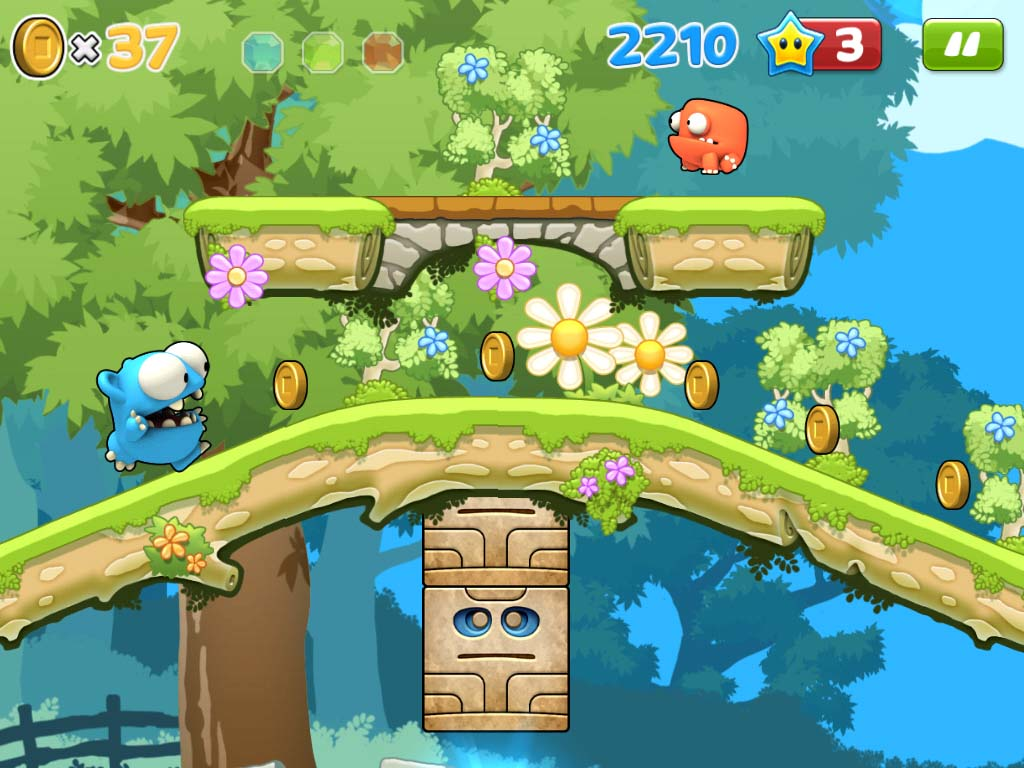
\includegraphics[clip= true, width= 0.8\columnwidth, trim= 1.5cm 3.0cm 0.6cm 0.0cm]{images/gameDesign/01_megarun.jpg}
	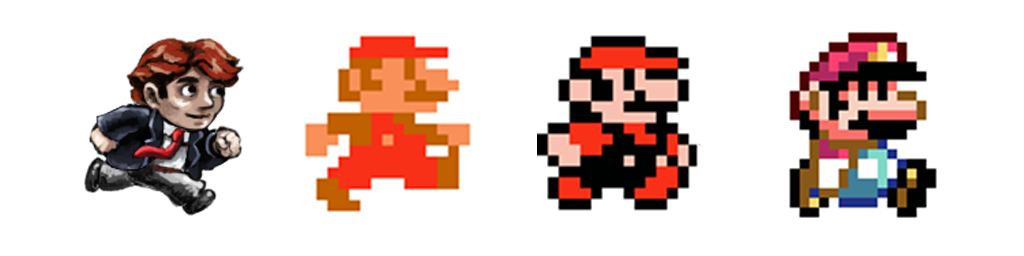
\includegraphics[width= 0.9\columnwidth]{images/gameDesign/02_braid_SM.jpg}
	\caption{Proporzione del personaggio di un platform game: Braid e SuperMario.}
	\label{fig:platform_proportions}
\end{figure}

Caratteristici dei platform sono quegli elementi di gioco che richiedono soprattutto delle abilità di reazione e concentrazione del giocatore, come corsa, salto o usare piattaforme.

Per quanto riguarda il movimento del personaggio, abbiamo deciso di ricorrere ad una corsa bidirezionale, a velocità uniforme in entrambe le direzioni ed indipendente dalla pressione del tasto di riferimento o dell’inclinazione della levetta analogica del controller. Questo assicura un padroneggiamento più veloce della meccanica, che, per le caratteristiche di gioco, non richiede una eccessiva complessità.
La velocità massima di corsa è raggiunta in maniera non esattamente istantanea, questo per assicurarsi un movimento non troppo brusco e quindi poco intuitivo.

La bidirezionalità fa sì che il personaggio si giri nel caso venga indicato un movimento opposto rispetto all’attuale direzione. Questo permette di raggiungere di nuovo, dove permesso dal design dei livelli, posti già visitati in precedenza (Figura~\ref{fig:platform_corsa}). Tale scelta non deve essere presa in maniera superficiale, in quanto ci si deve assicurare che elementi di gioco, incontrati in differenti momenti della partita, non si interfaccino in maniera problematica tra di loro. 
\begin{figure}%[h]
	\centering
	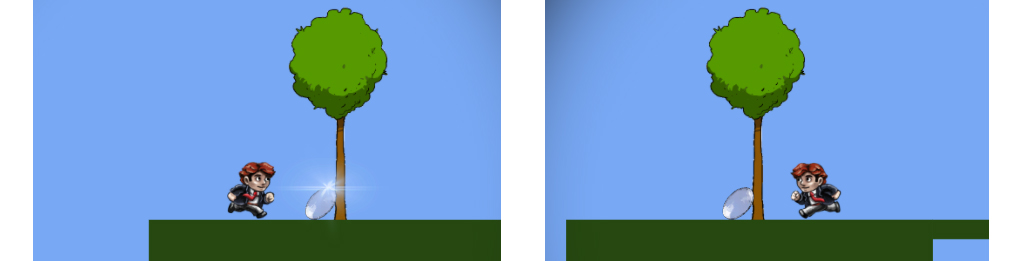
\includegraphics[width= \columnwidth]{images/gameDesign/03.jpg}
	\caption{Movimenti di corsa nel prototipo sviluppato}
	\label{fig:platform_corsa}
\end{figure}
In SuperMario Bros. (riferimento?) il personaggio può cambiare direzione, ma la camera non può tornare indietro, quindi, quando il personaggio arriva al bordo sinistro, è come se sbatta contro un muro invisibile.
La tipologia di gioco definita \textit{Endless Runner} invece, evita il problema impedendo al giocatore di invertire la direzione, nella maggior parte dei casi imponendo una corsa indipendente dall’input del giocatore o in altri casi semplicemente rallentabile o accelerabile (Figura~\ref{fig:platform_corsa_reali}).

\begin{figure}%[h]
	\centering
	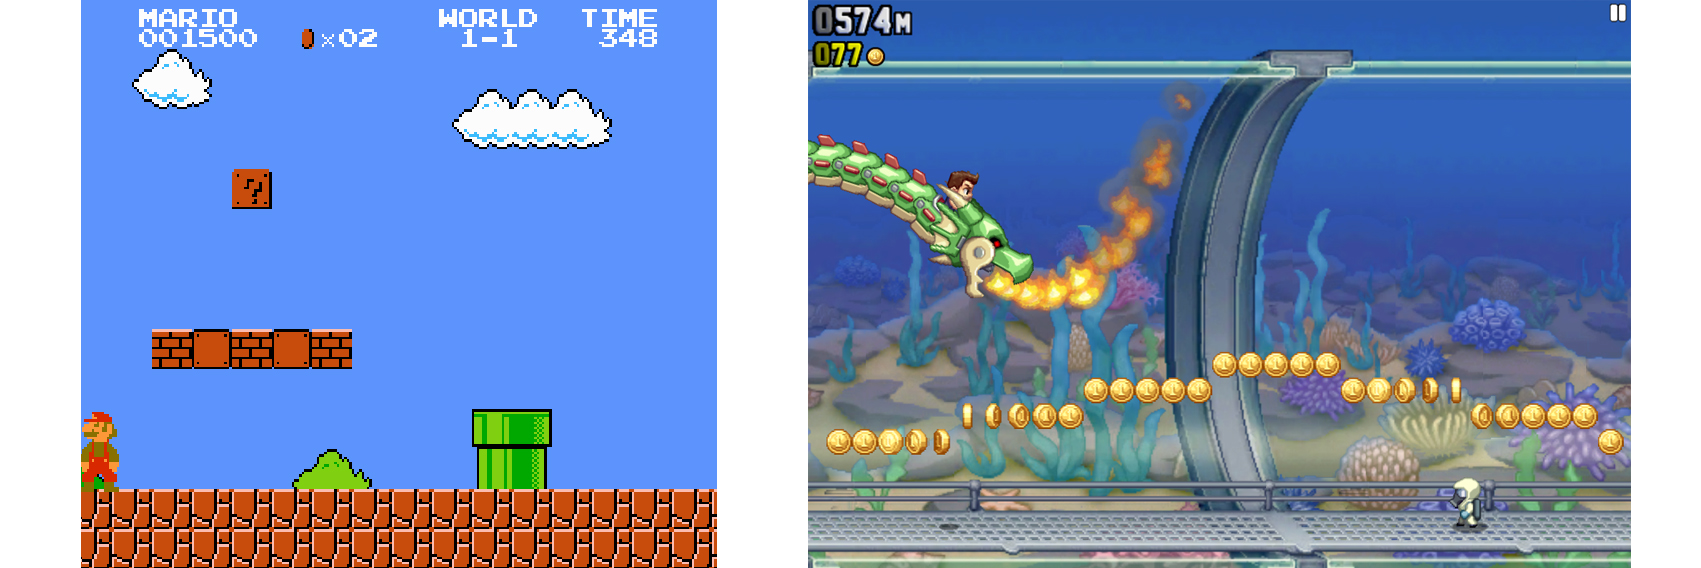
\includegraphics[width= \columnwidth]{images/gameDesign/04.jpg}
	\caption{Esempi di corsa: SuperMario e JetpackJoyride.}
	\label{fig:platform_corsa_reali}
\end{figure}

Per il salto, abbiamo deciso inizialmente di assegnare al personaggio una forza fissa verso l’alto, in seguito alla pressione del relativo bottone. Alcuni videogiochi invece assegnano una forza dipendente in maniera proporzionale dalla pressione del giocatore. Sono chiaramente due approcci differenti, il secondo fa sì che il salto sia una meccanica più complessa da padroneggiare, ma assicura delle possibilità di gameplay in più.
Durante i testing effettuati, abbiamo notato delle frequenti difficoltà nell’effettuare i salti, possiamo perciò pensare di prendere provvedimenti in tal senso, magari dando al giocatore un maggior controllo sulla potenza di salto, o limitando le sezioni in cui l’utilizzo del salto risulti troppo cruciale.

I movimenti del personaggio in aria sono controllabili attraverso i tasti direzionali. Perciò, dopo il salto o in seguito ad una caduta, il giocatore può direzionare o aggiustare la traiettoria di discesa. Non tutti i videogiochi platform assicurano tale comportamento, ma abbiamo ritenuto potesse essere utile per non frustrare eccessivamente il giocatore in seguito ad un salto non perfettamente calibrato al momento dello stacco.
La caduta del personaggio è soggetta ad una gravità 3 volte superiore al normale, è un elemento già presente in \textit{SuperMario} e ampiamente utilizzato nei giochi del genere per garantire una sensazione di repentinità al giocatore. La velocità di caduta è comunque limitata per garantirne il controllo.

\begin{figure}%[h]
	\centering
	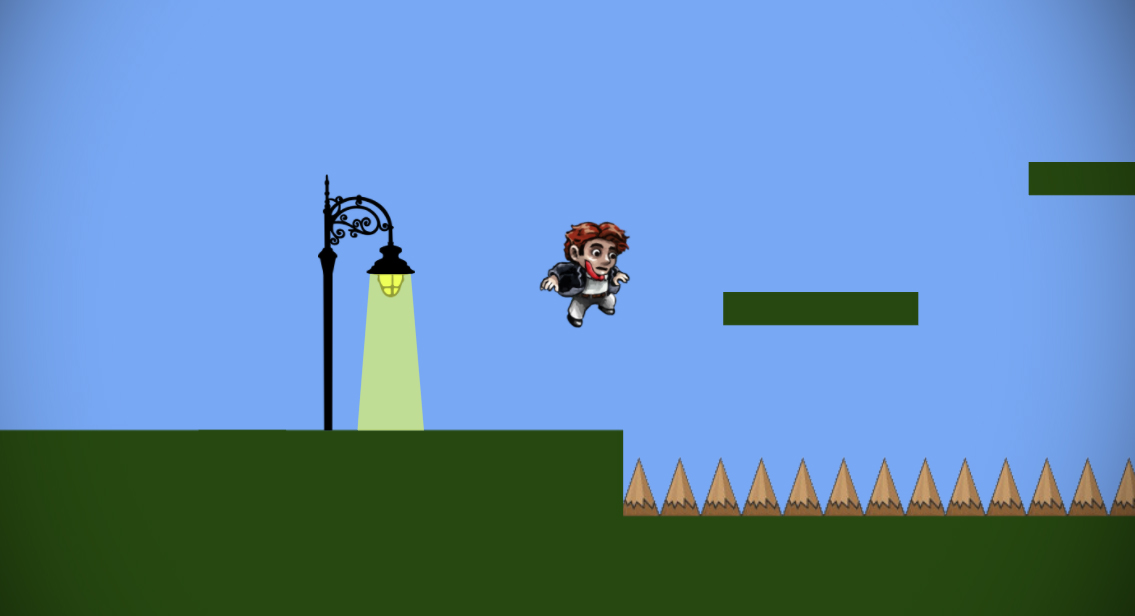
\includegraphics[width= 0.8\columnwidth]{images/gameDesign/05.jpg}
	\caption{Personaggio del prototipo, durante un salto.}
	\label{fig:platform_salto}
\end{figure}

Oltre alle meccaniche di corsa e salto, abbiamo dato la possibilità al personaggio di salire e scendere le scale. Questa è una meccanica non essenziale, che non aggiunge possibilità rispetto a quelle che non possa garantire una serie di salti, ma garantisce una maggiore sensazione di libertà al giocatore e permette una maggiore pulizia per quanto riguarda il level design. Le scale infatti, come mostrato in Figura~\ref{fig:platform_scala_piattaforme}, consentono di raggiungere luoghi per cui, altrimenti sarebbero state necessarie numerose piattaforme, che avrebbero potuto rendere la realizzazione dei livelli molto difficoltosa e confusa.

\begin{figure}%[h]
	\centering
	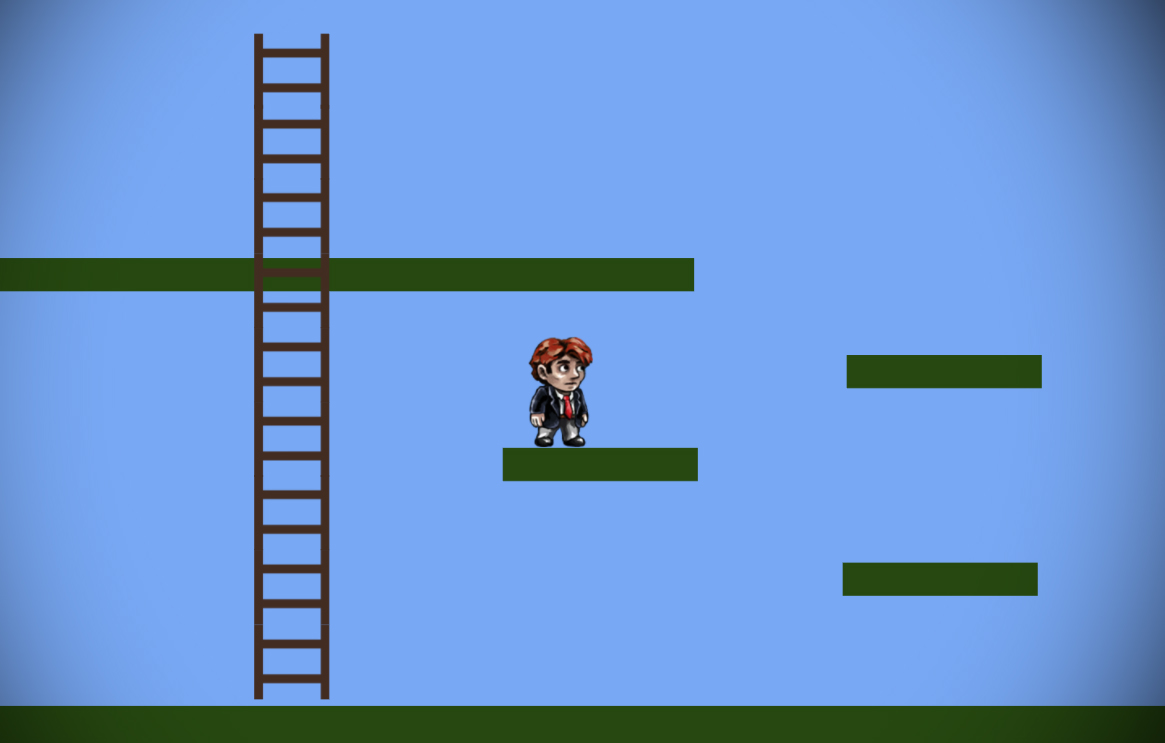
\includegraphics[width= 0.8\columnwidth]{images/gameDesign/06.jpg}
	\caption{Confronto tra utilizzo di scale e piattaforme equivalenti.}
	\label{fig:platform_scala_piattaforme}
\end{figure}

Le meccaniche di salto, controllo del personaggio in aria ed utilizzo scale sono state ispirate dal videogioco Braid (riferimento?), anche qui infatti il salto fornisce una forza indipendente dalla pressione del tasto e la possibilità di controllare il personaggio in caduta è una meccanica importante di gioco, anche se, rispetto a Braid, la forza impressa dal salto risulta meno forte e la gravità in caduta più espressiva, i movimenti in Braid appaiono più naturali, nel nostro caso invece più repentini ed eccessivi.

Sono state incluse nel gioco anche delle piattaforme mobili (Figura~\ref{fig:platform_piattaforme_mobili}). Queste hanno un movimento lineare tra due punti, uno dei quali raggiungibile dal personaggio, mentre l’altro si pone come obiettivo finale del movimento. Sono un elemento che mette alla prova le abilità di tempismo e di concentrazione del giocatore. Tali piattaforme risultano attraversabili dal basso verso l’alto, questo per permettere una maggiore libertà di approccio all’utente.
Durante i test effettuati, abbiamo notato che, spesso, i giocatori fanno fatica a comprendere i momenti esatti in cui la piattaforma cambia di direzione. Si sta perciò valutando se, nel prodotto finale non possa essere utile introdurre degli elementi che, graficamente, rappresentino dei limiti di inizio e fine corsa.

\begin{figure}%[h]
	\centering
	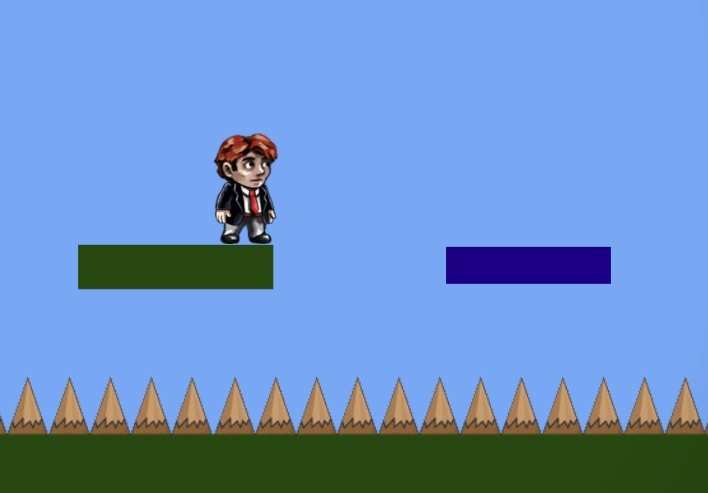
\includegraphics[width= 0.6\columnwidth]{images/gameDesign/07.jpg}
	\caption{Esempio di piattaforme mobili sviluppate.}
	\label{fig:platform_piattaforme_mobili}
\end{figure}

Graficamente, abbiamo deciso di rappresentare il terreno normale con una colorazione verde. Tale elemento non è attraversabile in nessuna direzione. Il personaggio collide sempre con esso.

Le piattaforme mobili vengono invece rappresentate con una colorazione blu scura, come si può osservare in Figura~\ref{fig:platform_piattaforme_mobili}.

Un altro terreno, che abbiamo deciso di sviluppare, permette di essere attraversato in entrambe le direzioni, ma solo se il personaggio sta utilizzando una scala. Permette appunto di attraversare terreni normalmente non attraversabili, ma caratterizzati dalla presenza della scala. La colorazione per questo tipo di terreno rimane comunque quella verde. Abbiamo verificato, tramite test e prototipazione, che questa scelta non influisce sulla comprensibilità della meccanica, in quanto caratterizzata dalla presenza della scala.

Parallelamente abbiamo ritenuto necessario sviluppare una tipologia differente di terreno, che permette di essere superato dal basso, ad esempio con un salto del personaggio. Non è attraversabile dall’alto. Tale scelta apre la strada ad una nuova meccanica, in quanto realizza una via a “senso unico” che può essere utile in fase di level design. Questo terreno invece, è differenziato dal resto tramite una colorazione blu più tenue rispetto alle piattaforme mobili.

Le 3 tipologie di terreno possono essere osservate in Figura~\ref{fig:platform_terreni}.

\begin{figure}%[h]
	\centering
	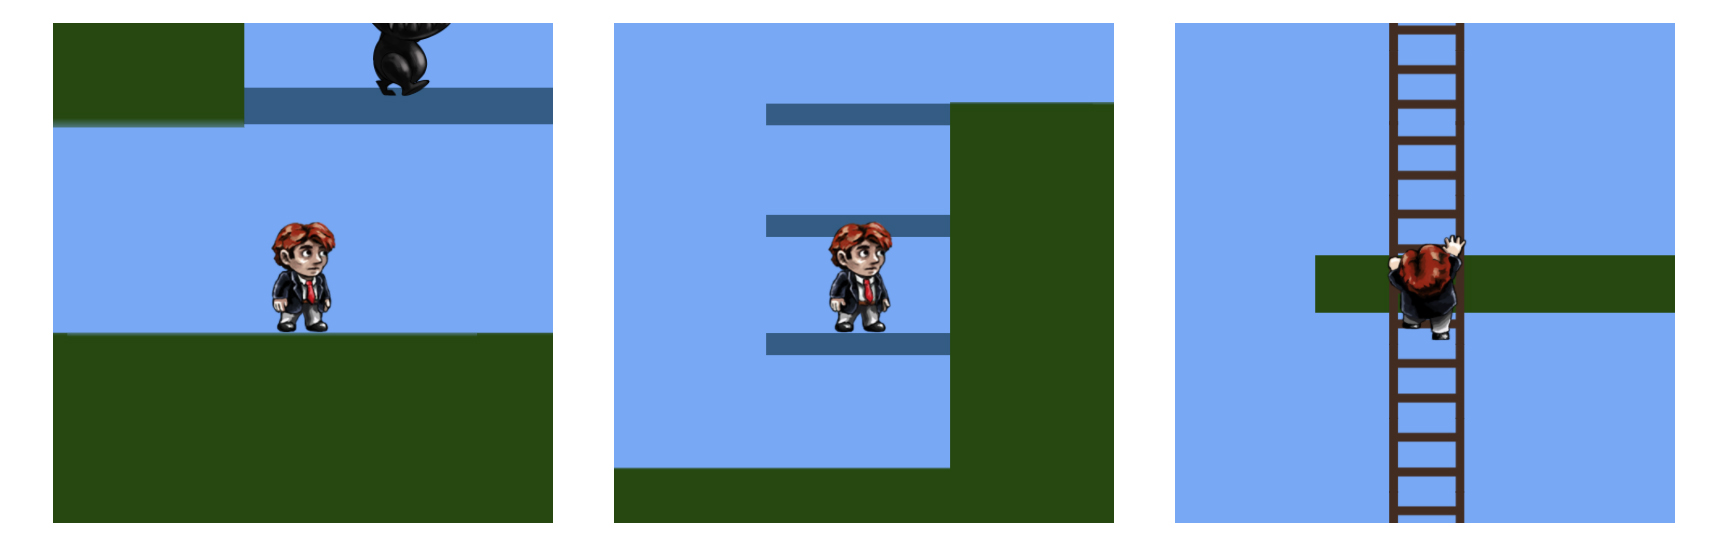
\includegraphics[width= \columnwidth]{images/gameDesign/08.jpg}
	\caption{Esempi delle tre tipologie di terreno sviluppate.}
	\label{fig:platform_terreni}
\end{figure}

\subsection{Elementi Puzzle}
\label{elementi_puzzle}

Oltre alle meccaniche Platform, che richiedono soprattutto reattività, tempismo e concentrazione del giocatore, il videogioco presenta anche caratteristiche tipiche del genere dei \textit{Puzzle Games}.

Questa categoria di videogiochi enfatizza soprattutto la risoluzione di enigmi e puzzles. Il giocatore deve perciò possedere le capacità di osservare la situazione in cui si trova il personaggio, analizzarne gli elementi, e capire in che modo debbano essere sfruttati ed usati per superare una determinata sezione o raggiungere un obiettivo.
Sono perciò richieste quelle che il libro \textit{The Art Of Game Design}\cite{artOfGameDesign} Definisce come abilità mentali (\textit{Mental Skills}):
“Le abilità mentali includono le capacità di memoria, osservazione e risoluzione di puzzle. Sebbene alcune persone evitino giochi che richiedono troppo impegno per quanto riguarda queste capacità, è raro che i giochi non le includano anche in piccola parte, perché i giochi sono interessanti quando ci sono decisioni interessanti da prendere, e prendere decisioni è una abilità mentale.”

Risulta necessario specificare che, nella fase di Level Design, abbiamo fatto particolare attenzione nel mescolare intelligentemente elementi platform e puzzle, in modo da essere in sintonia tra loro, senza che uno dei due elementi apparisse predominante sull’altro e che l’esperienza non risultasse eccessivamente frenetica e frustrante da un lato o lenta e noiosa dall’altro.
Le dinamiche puzzle ci hanno permesso anche di fare design riguardo il possibile utilizzo di strumenti particolari del pre-Cinema in maniera originale e curiosa (riferimento al capitolo), inserendo quindi elementi di gioco non presenti in altri esponenti del settore.
Elementi classici del puzzle game, che abbiamo inserito sono, ad esempio, leve, pulsanti, casse, porte, bilance e sequenze di bottoni.

Le leve (Figura~\ref{fig:platform_leve}) sono utilizzate per avere un effetto diretto sullo scenario di gioco. Generalmente, le abbiamo utilizzate per spostare elementi dell’ambientazione o attivare meccanismi.

\begin{figure}%[h]
	\centering
	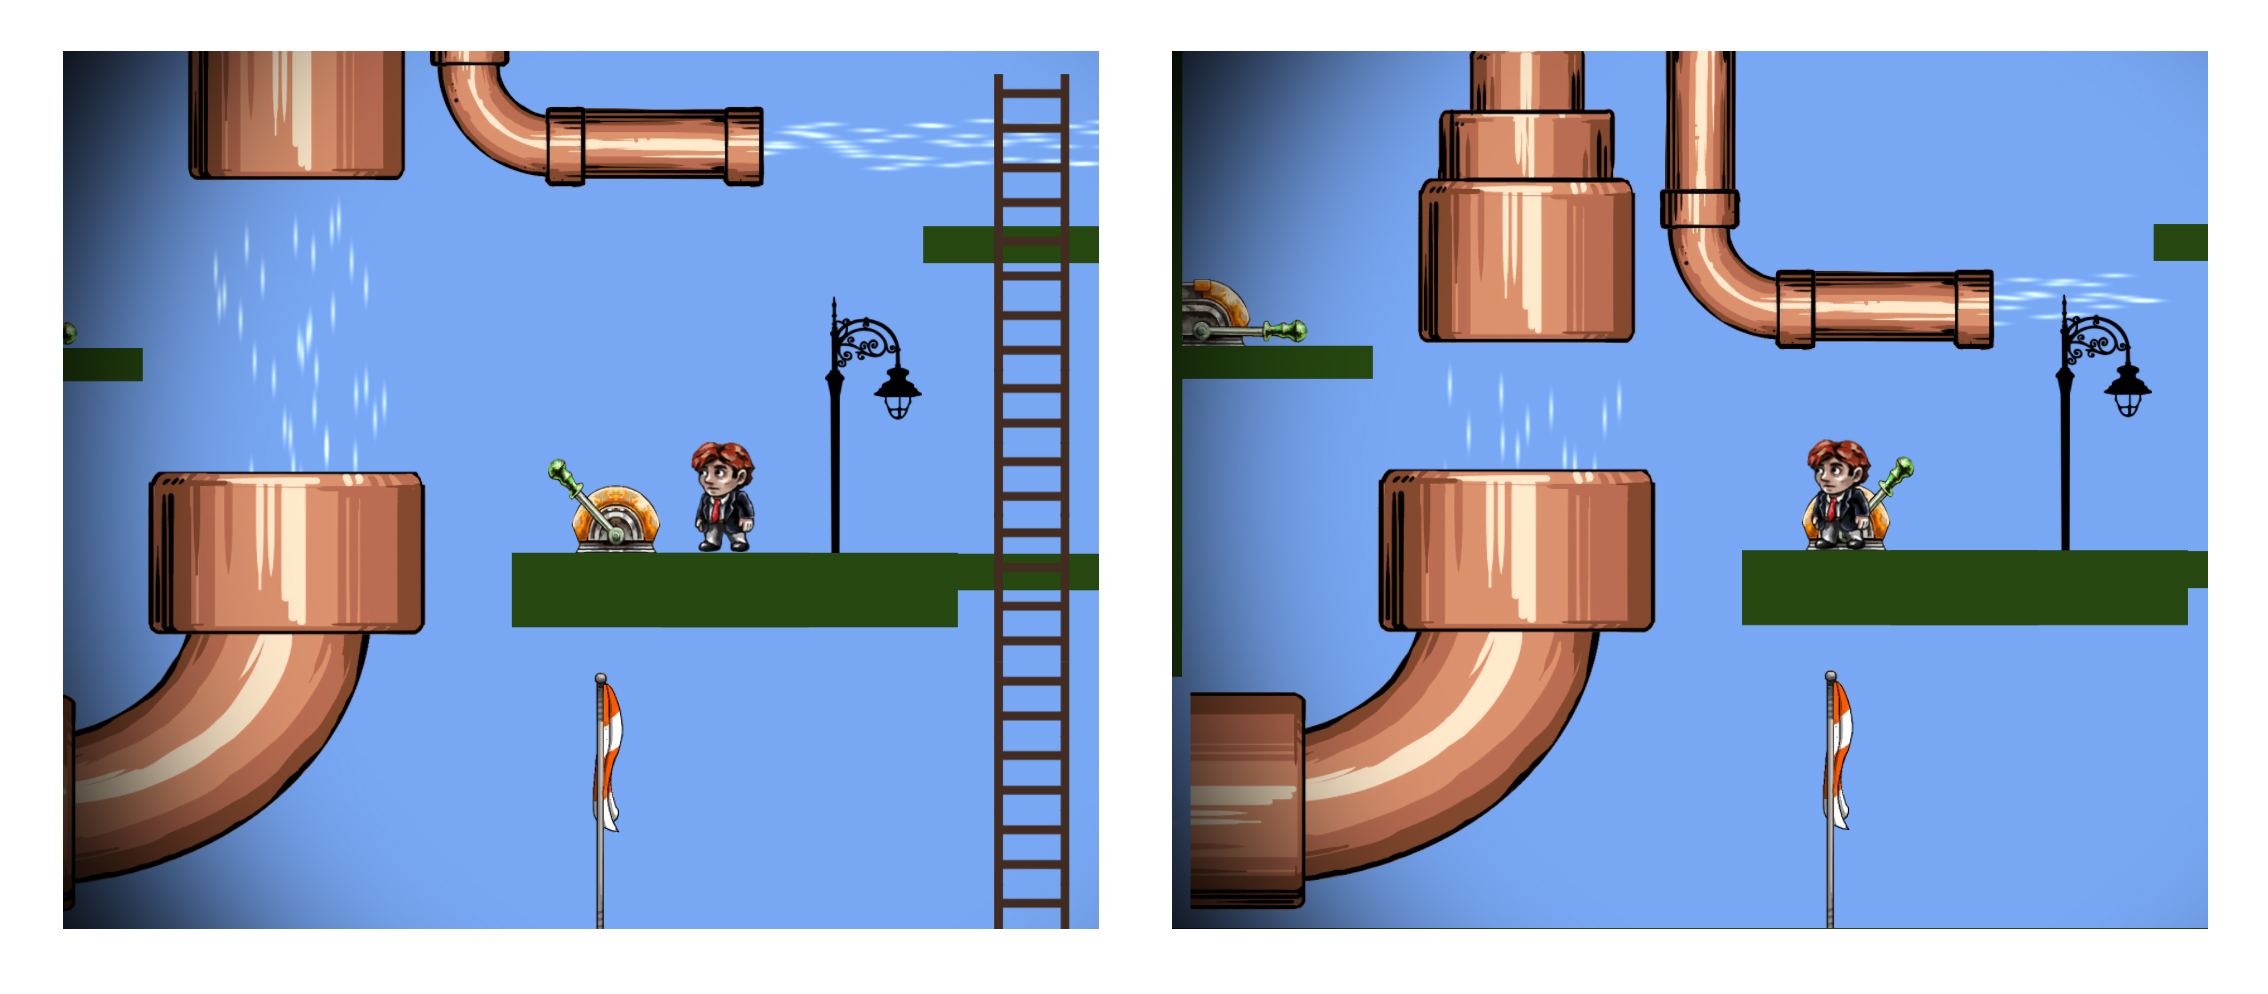
\includegraphics[width= \columnwidth]{images/gameDesign/09.jpg}
	\caption{Esempio di leva. Utilizzata per interagire con un elemento dello scenario.}
	\label{fig:platform_leve}
\end{figure}

I pulsanti a pressione possono essere intesi, concettualmente, come le leve, hanno un effetto immediato su alcuni elementi dello scenario. Nel nostro caso in particolare, abbiamo preferito associarli ad aperture e chiusure di porte, portoni o elementi traslabili che impediscono o permettono il passaggio del personaggio da una zona all’altra di gioco. Questa scelta è stata fatta per permettere al giocatore di capire immediatamente l’effetto di un bottone, spesso anche prima di premerlo.

L’attivazione dei bottoni avviene nel momento in cui il personaggio sale su di essi, hanno perciò un funzionamento a pressione. L’effetto diretto avviene al momento dell’attivazione. Quando il personaggio scende, i bottoni possono disattivarsi e quindi invertire l’effetto sortito sullo scenario di gioco o rimanere attivi e mantenere l’effetto nel tempo. Tale scelta dipende dal particolare utilizzo e quindi da scelte di level design.

I bottoni, come già specificato, vengono attivati dalla pressione su di essi, sia che venga applicata dal personaggio principale, che da un nemico (riferimento al capitolo). Come mostrato in Figura~\ref{fig:platform_bottoni} abbiamo comunque ritenuto utile inserire delle casse come elemento di gioco. Esse permettono di premere i bottoni senza la presenza del personaggio, oltre che salirci sopra per raggiungere posti più elevati.

\begin{figure}%[h]
	\centering
	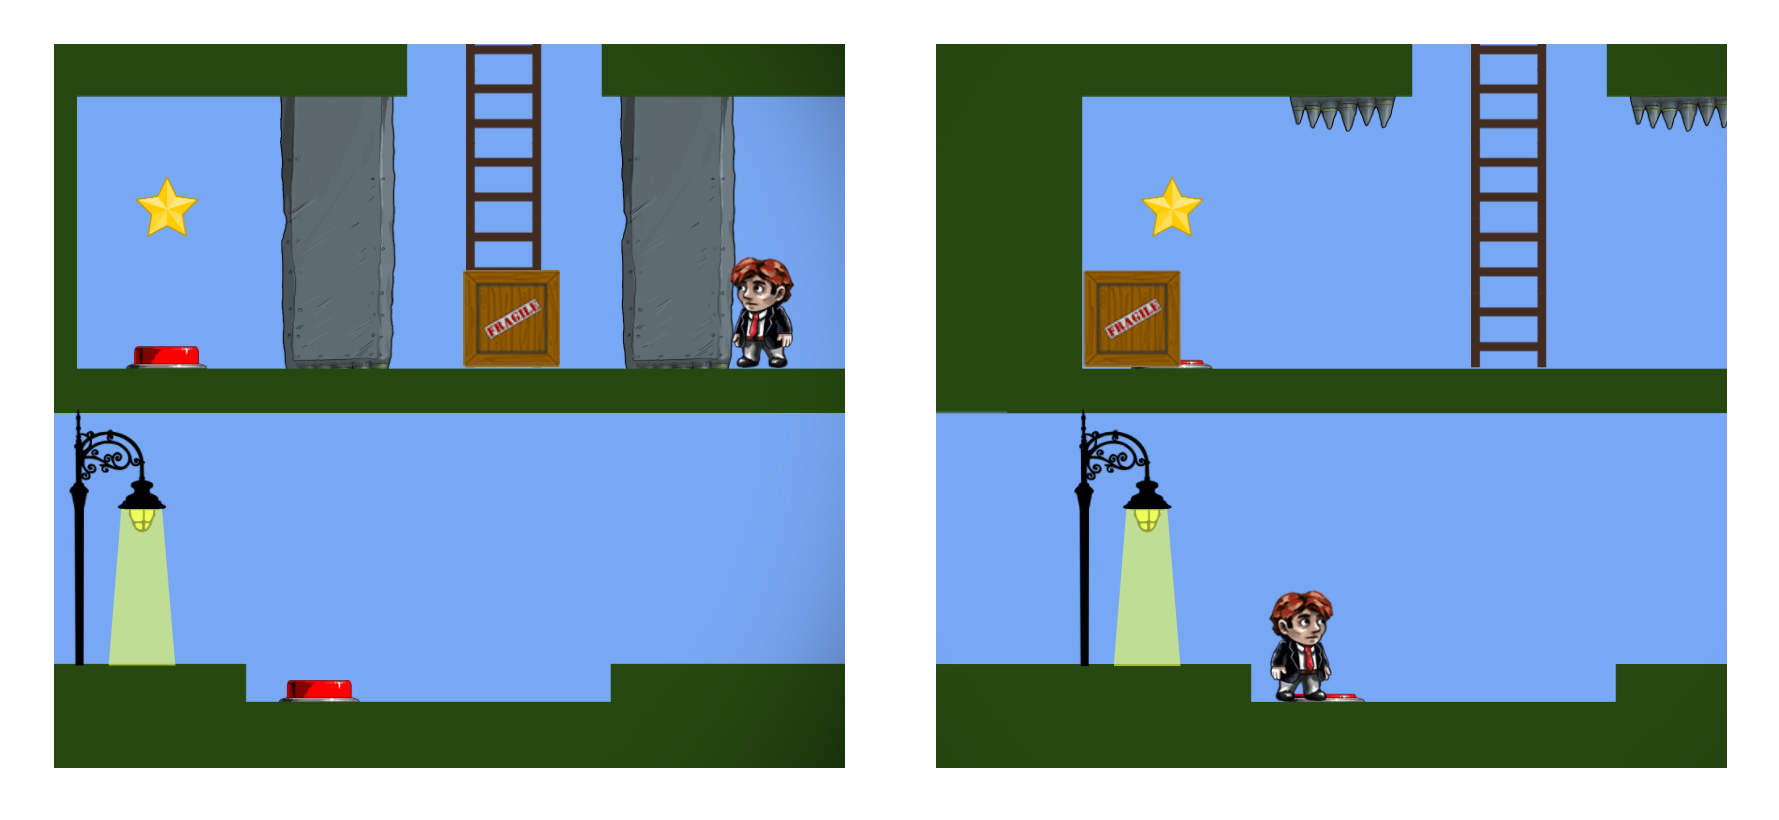
\includegraphics[width= \columnwidth]{images/gameDesign/10.jpg}
	\caption{Bottoni premuti da casse.}
	\label{fig:platform_bottoni}
\end{figure}

Coerentemente con il concetto di pressione e pesi, abbiamo introdotto nel gioco anche delle bilance (Figura~\ref{fig:platform_bilancia}). Per semplicità, abbiamo ipotizzato che ogni elemento di gioco abbia una massa, relativamente alla bilancia, di una unità. Ipotizzando perciò che in un piatto ci sia una cassa, per avere una situazione di equilibro, è sufficiente che sull’altro piatto ci sia il personaggio. La bilancia, come le leve, permette di attivare un elemento dello scenario. È stata utilizzata, ad esempio, per un enigma in cui è necessario spostare un numero di nemici sufficienti in un piatto, per far sì che l’altro si alzi e attivi un bottone.

\begin{figure}%[h]
	\centering
	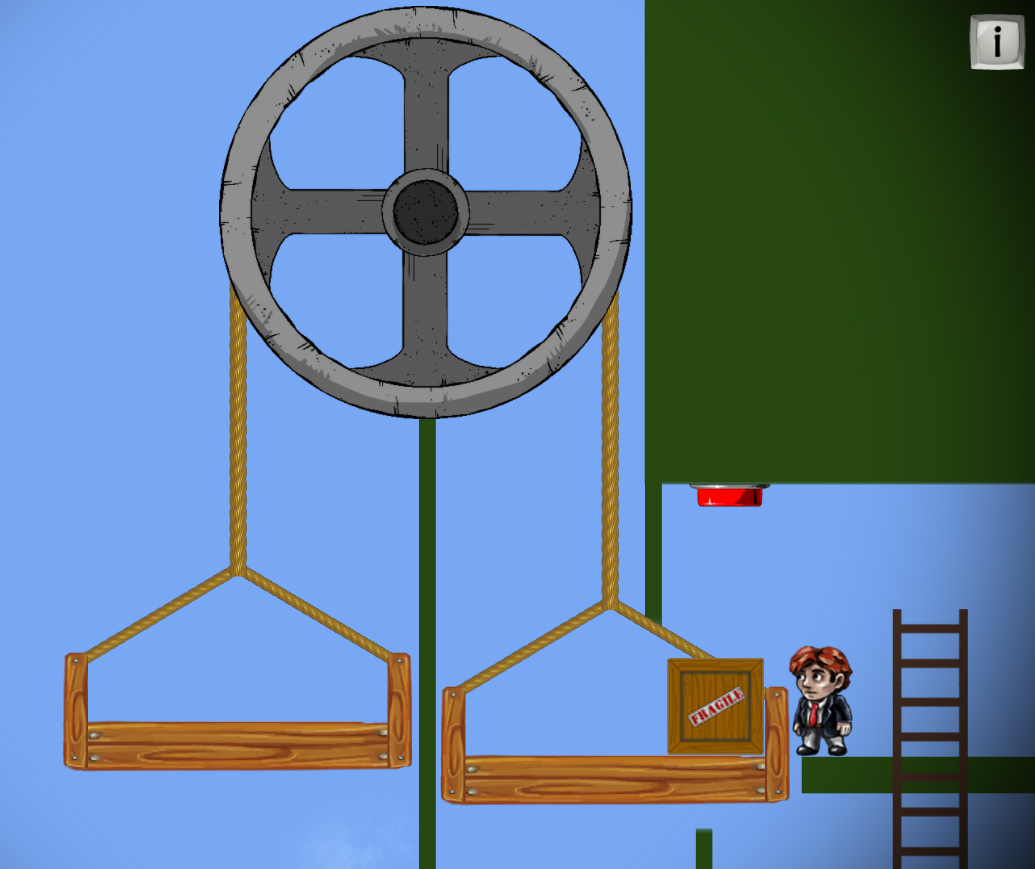
\includegraphics[width= 0.5\columnwidth]{images/gameDesign/11.jpg}
	\caption{Bilancia.}
	\label{fig:platform_bilancia}
\end{figure}

Un altro elemento interessante sono le sequenze di bottoni (Figura~\ref{fig:platform_sequenza_bottoni}
). Queste hanno lo stesso funzionamento dei bottoni singoli ma, per interagire con una porta è necessario attivarli tutti nella giusta sequenza. Se il primo bottone premuto è quello giusto, questo rimane attivo, se il secondo non è giusto, vengono disattivati tutti e la sequenza deve ricominciare dall’inizio. Quando vengono premuti tutti i bottoni nella giusta sequenza, viene attivato l’elemento dello scenario prestabilito, nel nostro caso le sequenze di bottoni sono sempre state utilizzate per aprire porte.

\begin{figure}%[h]
	\centering
	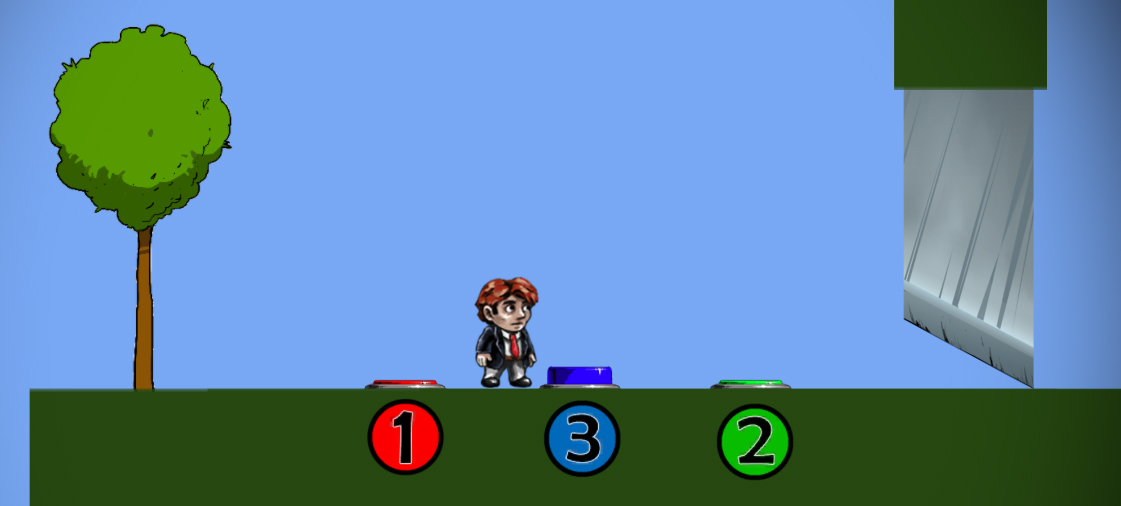
\includegraphics[width= 0.7\columnwidth]{images/gameDesign/12.jpg}
	\caption{Sequenza di bottoni.}
	\label{fig:platform_sequenza_bottoni}
\end{figure}

Viene riportata di seguito l’analisi di un enigma presente in uno dei livelli sviluppati. Nella figura \ref{fig:platform_enigma} si possono notare alcuni elementi non ancora analizzati, come il nemico, la lanterna magica o la stella, fare riferimento ai relativi capitoli (riferimenti) per approfondimenti sul loro utilizzo, che qui verrà spiegato in maniera superficiale.

\begin{figure}%[h]
	\centering
	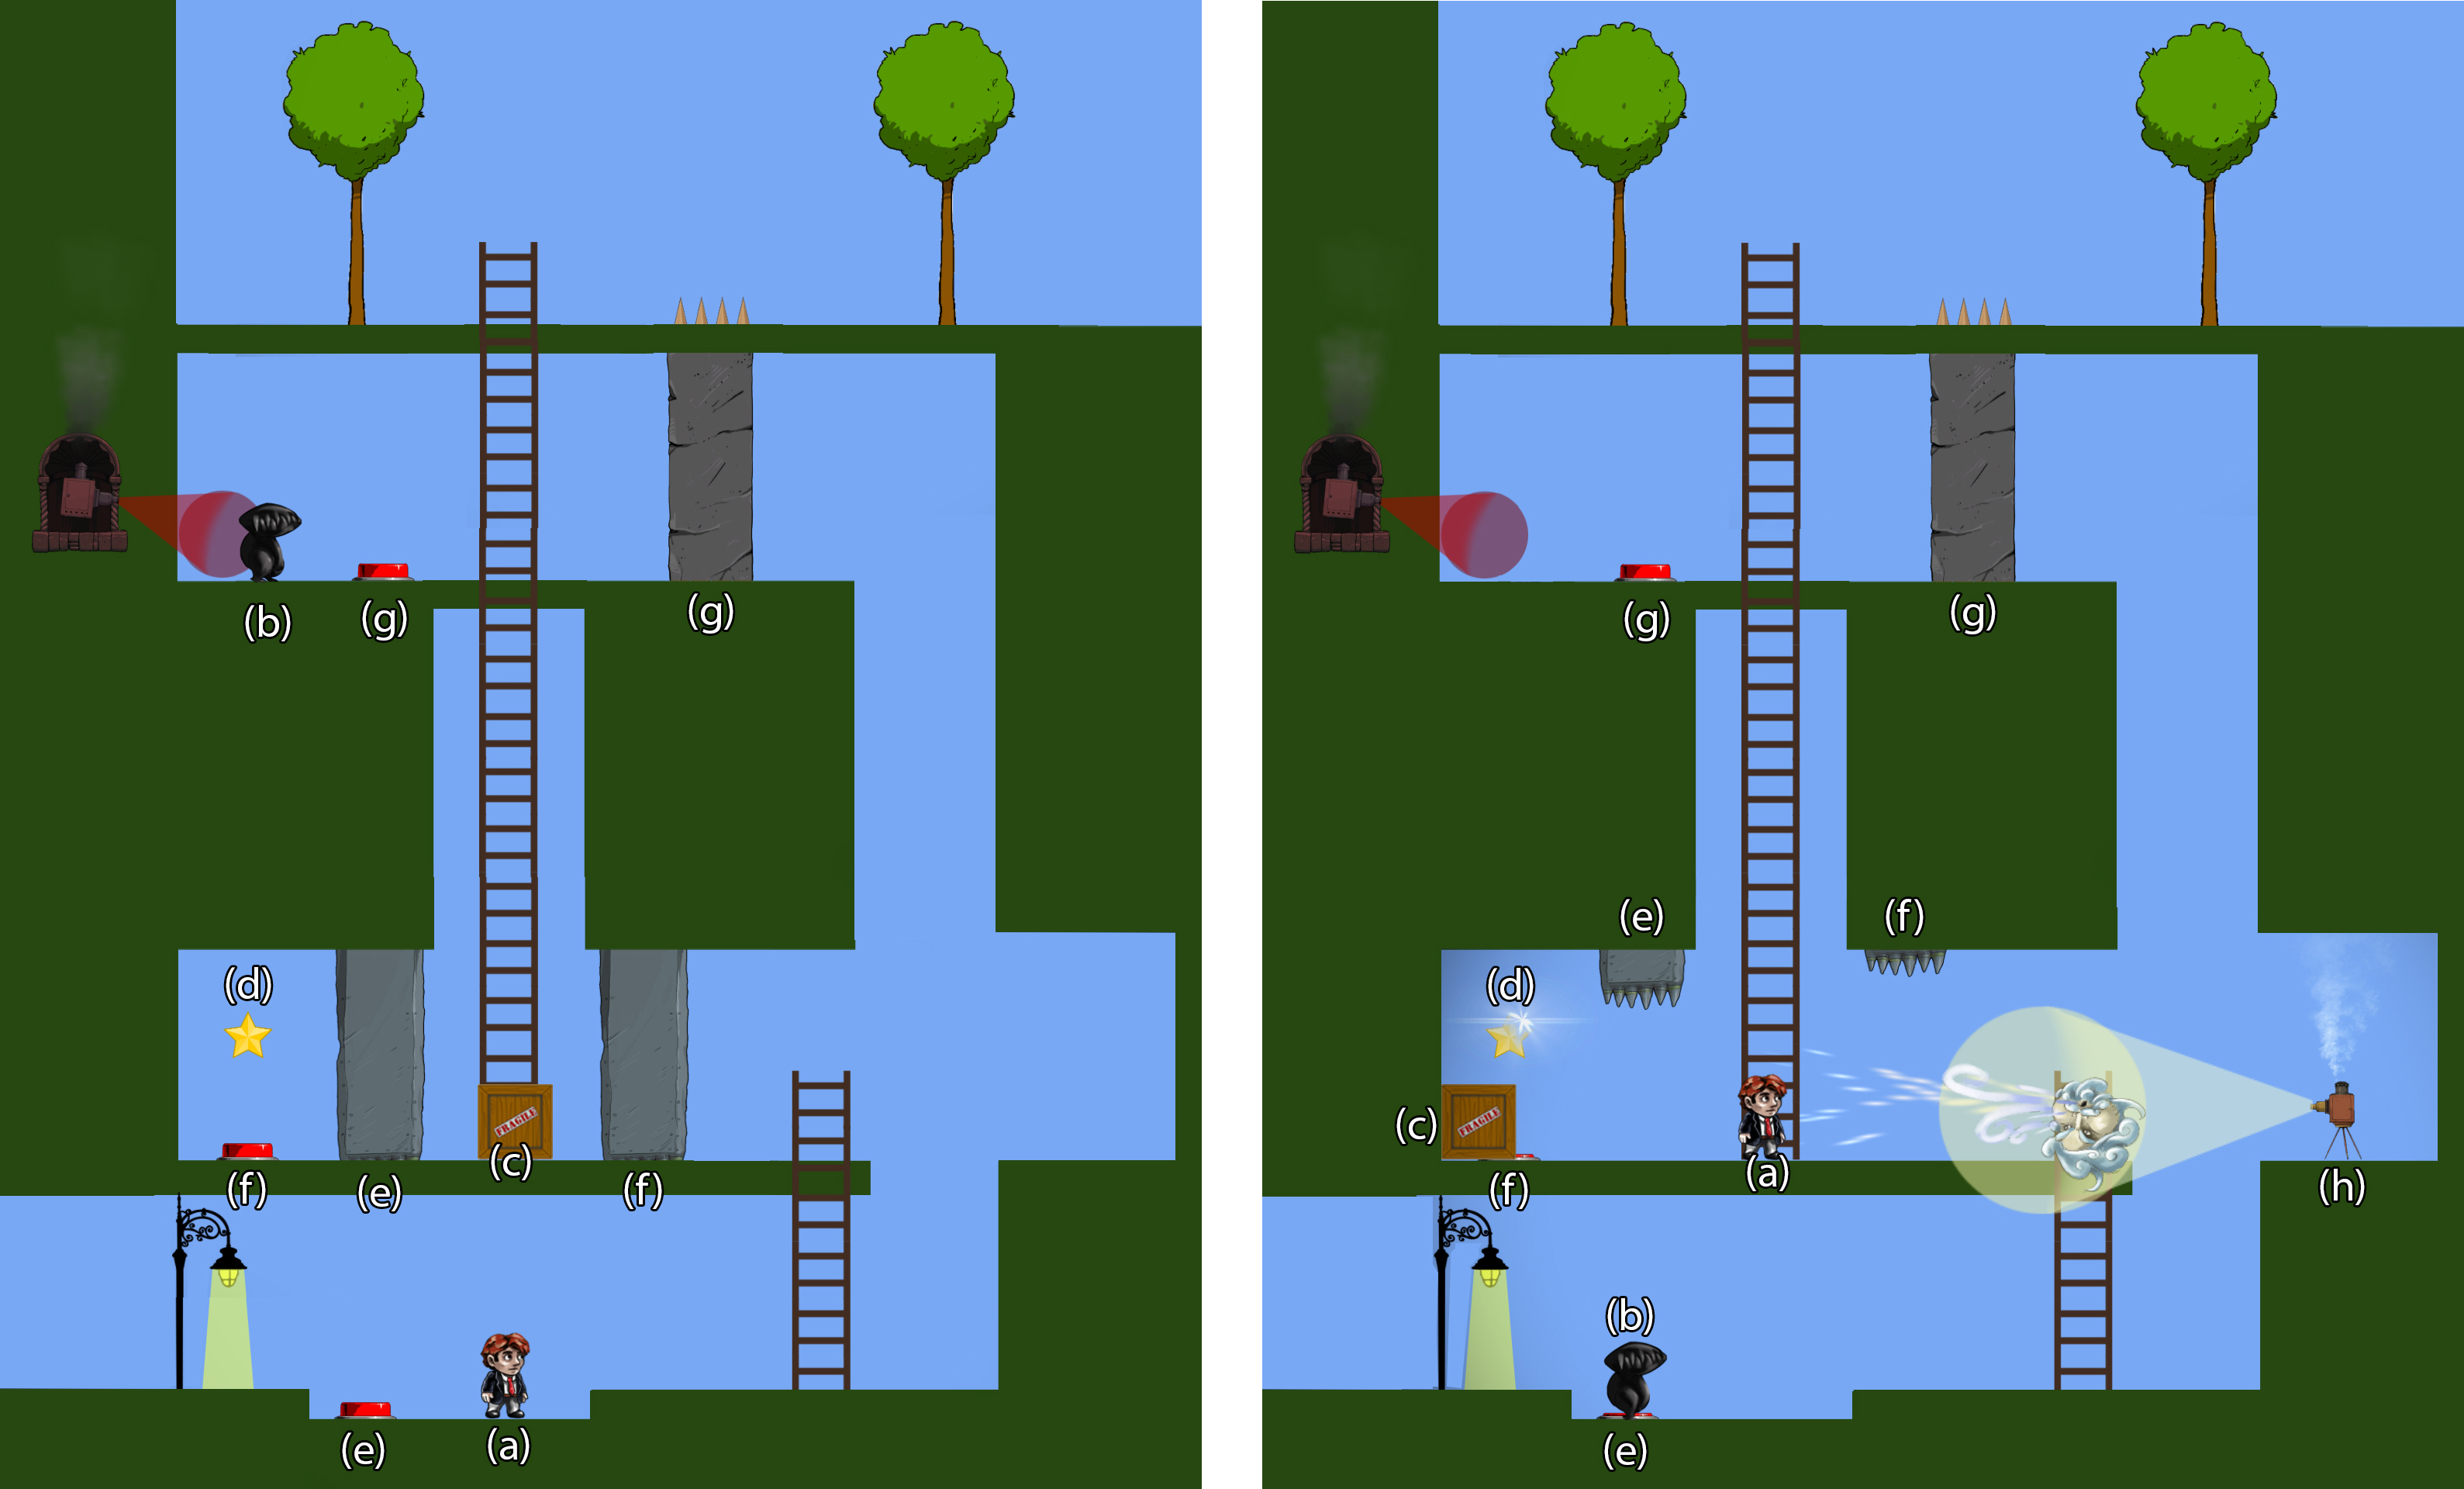
\includegraphics[width= \columnwidth]{images/gameDesign/13.jpg}
	\caption{Esempio di enigma.}
	\label{fig:platform_enigma}
\end{figure}

Come spesso avviene nei vari livelli sviluppati, la via per proseguire non richiede la completa risoluzione dell’enigma, ma solo la parte più semplice di esso, così da permettere, anche ai giocatori non interessati al raccoglimento di tutti i collezionabili, di proseguire con la partita.
In figura~\ref{fig:platform_enigma} vengono contrassegnati con la stessa lettera i bottoni e le relative porte che vengono azionate.

Il personaggio può subito porsi sopra il bottone “e” e notare l’apertura della relativa porta, che conduce ad una stanza con un altro bottone. Il giocatore capisce che la pressione di questo bottone è l’unico modo per proseguire. Raggiunge perciò un luogo favorevole per piazzare a terra la lanterna magica e sfruttarne il vento prodotto per spingere la cassa, bloccata però dalla porta “e”. Il personaggio deve quindi tornare sul bottone “e” e permettere alla cassa di premere il bottone “f”. Il personaggio può quindi raggiungere le scale e salire. Il nemico, premendo il pulsante “g”, attiva una porta con degli spuntoni, che blocca il raggiungimento dell’uscita, posta nella zona in alto a destra dell’immagine. Si deve perciò fare attenzione ad avere il giusto tempismo.

Come si può notare dall’immagine, il personaggio principale può quindi raggiungere l’uscita, ma rimane una stella da raccogliere. Come già specificato, solo la parte obbligatoria dell’enigma è stata risolta, ma non quella opzionale per il raccoglimento della stella.

Il giocatore può quindi, una volta salita la scala ed arrivati sul livello del nemico, scendere dalla scala, aspettare che il nemico si volti verso la porta/macigno, saltare il nemico, premere il bottone “b” e permettere così al nemico di cadere al piano inferiore. Questo, camminando, raggiungerà la zona con il bottone “e”, senza la possibilità di uscirne. Continuerà perciò ad attivare la porta che conduce alla stanza con la stella, che potrà quindi essere agilmente raccolta dal personaggio. Una volta collezionata, si può proseguire lungo il livello.
La seconda immagine in Figura~\ref{fig:platform_enigma} mostra l’enigma completamente risolto.

\subsection{Camera e Puntatore}
\label{sec:camera_e_puntatore}

